\textbf{Beispiel 1}\\ \\
Freigeschnittenen Stäbe:
\begin{figure}[h]
	\centering
	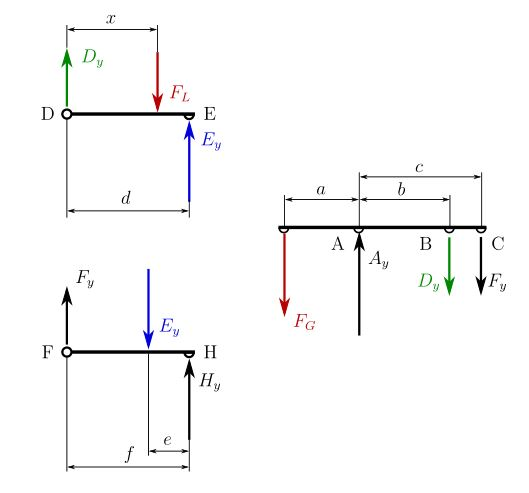
\includegraphics[width= 10cm]{tikz/13_07_2018_1}
\end{figure}
\newpage
\noindent
a)\\ \\
Die Gleichgewichtsgleichungen für den Stab D-E lauten
\begin{align*}
	\textbf{e}_y &: D_y + E_y - F_L = 0\\
	\textbf{e}_z &: E_yd - F_Lx = 0 
\end{align*}
Aus diesen folgen nun die Kräfte
\begin{align*}
	E_y &= F_L \frac{x}{d} \\
	D_y &= F_L \left(1 - \frac{x}{d}\right)
\end{align*}
b)\\ \\
Die Gleichgewichtsgleichungen für den Stab F-H lauten
\begin{align*}
	\textbf{e}_y &: F_y + H_y - E_y = 0\\
	\textbf{e}_z &: E_ye - F_yf = 0
\end{align*}
Aus diesen folgen nun die Kräfte
\begin{align*}
	F_y &= E_y \frac{e}{f} = F_L \frac{x}{d}\frac{e}{f} \\
	H_y &= E_y - F_y \\
		&= F_L \frac{x}{d}\left(1 - \frac{e}{f}\right)
\end{align*}
c)\\ \\
Die Gleichgewichtsgleichungen für den Stab A-B-C lauten
\begin{align*}
	\textbf{e}_y &: A_y - F_G - D_y - F_y = 0\\
	\textbf{e}_z &: F_Ga - D_yb - F_yc = 0
\end{align*}
Aus diesen folgen nun die Kräfte
\begin{align*}
	F_G &= D_y\frac{b}{a} + F_y\frac{c}{a} \\
		&= \frac{F_L}{a}\left[b - \frac{x}{d}\left(b - \frac{ec}{f}\right)\right] \\
	A_y &= F_L\left[\frac{b}{a} - \frac{x}{d}\left(\frac{b}{a} - \frac{ec}{af}\right) + 1 - \frac{x}{d}\left(1 - \frac{e}{f}\right)\right]
\end{align*}
d)\\ \\
Damit die geforderte Bedingung eingehalten werden kann, muss lautet das Längenverhältnis
\[
	\frac{b}{c} = \frac{e}{f}
\]
Dadurch gilt $F_G = F_L\frac{b}{a}$.